\chapter{Computing the non isomorphic MISs of the n-cycle graph}
\label{sec:24}

\abstract*{}

\abstract{}

Due to the public success of our common 2008 publication with Jean-Luc Marichal \citep{ISOMIS-08} , we present in this chapter an example Python session for computing the non isomorphic maximal independent sets (MISs) from the 12-cycle graph, i.e. a \texttt{CirculantDigraph} class instance of order 12 and symmetric circulants $1$ and $-1$.
\begin{lstlisting}
>>> from digraphs import CirculantDigraph
>>> c12 = CirculantDigraph(order=12,circulants=[1,-1])
>>> c12 # 12-cycle digraph instance
  *------- Digraph instance description ------*
   Instance class   : CirculantDigraph
   Instance name    : c12
   Digraph Order    : 12
   Digraph Size     : 24
   Valuation domain : [-1.0, 1.0]
   Determinateness  : 100.000
   Attributes       : ['name', 'order', 'circulants',
                       'actions', 'valuationdomain',
                       'relation', 'gamma', 'notGamma']
\end{lstlisting}

Such $n$-cycle graphs are also provided as undirected graph instances by the \texttt{CycleGraph} class.
\begin{lstlisting}
>>> from graphs import CycleGraph
>>> cg12 = CycleGraph(order=12)
>>> cg12
  *------- Graph instance description ------*
   Instance class   : CycleGraph
   Instance name    : cycleGraph
   Graph Order      : 12
   Graph Size       : 12
   Valuation domain : [-1.0, 1.0]
   Attributes       : ['name', 'order', 'vertices',
                       'valuationDomain', 'edges',
                       'size', 'gamma']
>>> cg12.exportGraphViz('cg12')
\end{lstlisting}
\begin{figure}[h]
\sidecaption
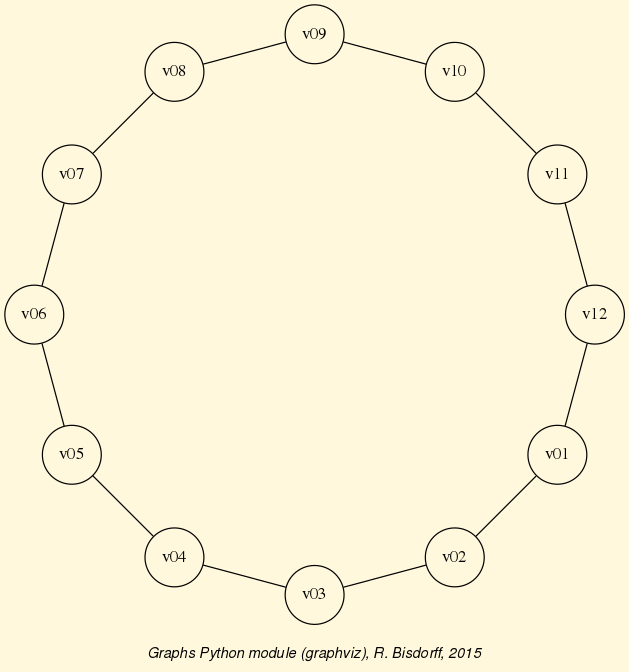
\includegraphics[width=6cm]{Figures/cg12.png}
\caption{The 12-cycle graph} 
\label{fig:24.1}       % Give a unique label
\end{figure}

\section{Computing maximal independent sets (MISs)}
\label{sec:24.1}
---------------------------------------------

A non isomorphic MIS corresponds in fact to a set of isomorphic MISs, i.e. an orbit of MISs under the automorphism group of the 12-cycle graph. We are now first computing all maximal independent sets that are detectable in the 12-cycle digraph with the \texttt{showMIS()} method.
\begin{lstlisting}
>>> c12.showMIS(withListing=False)
  *---  Maximal independent choices ---*
   number of solutions:  29
   cardinality distribution
   card.:  [0, 1, 2, 3, 4,  5,  6, 7, 8, 9, 10, 11, 12]
   freq.:  [0, 0, 0, 0, 3, 24,  2, 0, 0, 0,  0,  0,  0]
   Results in c12.misset
\end{lstlisting}
In the 12-cycle graph, we observe 29 labelled MISs: 3 of cardinality 4, 24 of cardinality 5, and 2  of cardinality 6. In case of n-cycle graphs with $n$ > 20, as the cardinality of the MISs becomes big, it is preferable to use the shell \texttt{perrinMIS} command compiled from C and installed  along with all the \Digraph python modules for computing the set of MISs observed in the graph\footnote{The \texttt{perrinMIS} shell command may be installed system wide with the command texttt{make installPerrin} from the main \Digraph directory. It is stored by default into \texttt{/usr/local/bin/}. This may be changed with the \texttt{INSTALLDIR} flag. The command \texttt{make installPerrinUser} installs it instead without sudo into the user's private \texttt{.bin} directory.}.
\begin{lstlisting}
...$ echo 12 | /usr/local/bin/perrinMIS
  # $------------------------------------- #
  # Generating MIS set of Cn with the      #
  # Perrin sequence algorithm.             #
  # Temporary files used.                  #
  # even versus odd order optimised.       #
  # RB December 2006                       #
  # Current revision Dec 2018              #
  # -------------------------------------- #
  Input cycle order ? <-- 12
   mis 1 : 100100100100
   mis 2 : 010010010010
   mis 3 : 001001001001
    ...
    ...
    ...
   mis 27 : 001001010101
   mis 28 : 101010101010
   mis 29 : 010101010101
   Cardinalities:
   0 : 0
   1 : 0
   2 : 0
   3 : 0
   4 : 3
   5 : 24
   6 : 2
   7 : 0
   8 : 0
   9 : 0
   10 : 0
   11 : 0
   12 : 0
   Total: 29
   execution time: 0 sec. and 2 millisec.
\end{lstlisting}
Reading in the result of the \texttt{perrinMIS} shell command, stored in a file called by default \texttt{curd.dat}, may be operated with the \texttt{readPerrinMisset()} method.
\begin{lstlisting}
>>> c12.readPerrinMisset(file='curd.dat')
>>> c12.misset
    {frozenset({'5', '7', '10', '1', '3'}),
     frozenset({'9', '11', '5', '2', '7'}),
     frozenset({'7', '2', '4', '10', '12'}),
     ...
     ...
     ...
     frozenset({'8', '4', '10', '1', '6'}),
     frozenset({'11', '4', '1', '9', '6'}),
     frozenset({'8', '2', '4', '10', '12', '6'})
    }
\end{lstlisting}

\section{Computing the automorphism group}
\label{sec:24.2}

For computing the corresponding non isomorphic MISs, we actually need the automorphism group of the c12-cycle graph. The \texttt{Digraph} class therefore provides the \texttt{automorphismGenerators()} method which adds automorphism group generators to a \texttt{Digraph} class instance with the help of the external shell \texttt{dreadnaut} command from the \emph{nauty} software package \footnote{The \texttt{automorphismGenerators} method uses the \texttt{dreadnaut} shell command from the \emph{nauty} software package. See https://www3.cs.stonybrook.edu/~algorith/implement/nauty/implement.shtml . On Mac OS there exist dmg installers and on Ubuntu Linux or Debian, one may easily install it with \texttt{...\$ sudo apt-get install nauty}.}.
\begin{lstlisting}
>>> c12.automorphismGenerators()
      ...
    Permutations
    {'1':'1', '2':'12', '3':'11', '4':'10',
     '5':'9', '6':'8', '7':'7', '8':'6', '9':'5',
     '10':'4', '11':'3', '12':'2'}
    {'1':'2', '2':'1', '3':'12', '4':'11', '5':'10', 
     '6':'9', '7':'8', '8':'7', '9':'6', '10':'5', 
     '11':'4', '12':'3'}
>>> print('grpsize = ', c12.automorphismGroupSize)
   grpsize = 24
\end{lstlisting}
The 12-cycle graph automorphism group is generated with both the permutations above and has group size 24.

\section{Computing the isomorphic MISs}
\label{sec:24.3}

The \texttt{showOrbits()} method renders now the labelled representatives of each of the four orbits of isomorphic MISs observed in the 12-cycle graph (see Lines 7-10 below).
\begin{lstlisting}
>>> c12.showOrbits(c12.misset,withListing=False)
    ...
  *---- Global result ----
   Number of MIS:  29
   Number of orbits :  4
   Labelled representatives and cardinality:
   1: ['2','4','6','8','10','12'], 2
   2: ['2','5','8','11'], 3
   3: ['2','4','6','9','11'], 12
   4: ['1','4','7','9','11'], 12
   Symmetry vector
   stabilizer size: [1, 2, 3, ..., 8, 9, ..., 12, 13, ...]
   frequency      : [0, 2, 0, ..., 1, 0, ...,  1,  0, ...]
\end{lstlisting}
The corresponding group stabilizers' sizes and frequencies: orbit 1 with 6 symmetry axes, orbit 2 with 4 symmetry axes, and orbits 3 and 4 both with one symmetry axis (see Lines 12-13 above), are illustrated in the corresponding unlabelled graphs of Fig. \ref{fig:24.1} below.
\begin{figure}[h]
\sidecaption
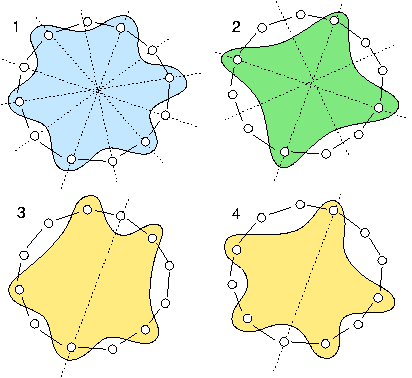
\includegraphics[width=6cm]{Figures/c12.png}
\caption{The symmetry axes of the four non isomorphic MISs of the 12-cycle graph} 
\label{fig:24.2}       % Give a unique label
\end{figure}

The non isomorphic MISs in the 12-cycle graph represent in fact all the ways one may write the number 12 as the circular sum of '2's and '3's without distinguishing opposite directions of writing. The first orbit corresponds to writing six times a '2'; the second orbit corresponds to writing four times a '3'. The third and fourth orbit correspond to writing two times a '3' and three times a '2'. There are two non isomorphic ways to do this latter circular sum. Either separating the '3's by one and two '2's, or by zero and three '2's (see \citep{ISOMIS-08}).
 
%%%%%%% The chapter bibliography
%\normallatexbib
\clearpage
\phantomsection
\addcontentsline{toc}{section}{Chapter Bibliography}
\bibliographystyle{dinat}
\typeout{}
\bibliography{03-backMatters/reference}
%\chapter{Computing the non isomorphic MISs of the n-cycle graph}
\label{sec:24}

\abstract*{}

\abstract{}

Due to the public success of our common 2008 publication with Jean-Luc Marichal [ISOMIS-08] , we present in this chapter an example Python session for computing the non isomorphic maximal independent sets (MISs) from the 12-cycle graph, i.e. a \texttt{CirculantDigraph} class instance of order 12 and symmetric circulants $1$ and $-1$.
\begin{lstlisting}
>>> from digraphs import CirculantDigraph
>>> c12 = CirculantDigraph(order=12,circulants=[1,-1])
>>> c12 # 12-cycle digraph instance
  *------- Digraph instance description ------*
   Instance class   : CirculantDigraph
   Instance name    : c12
   Digraph Order    : 12
   Digraph Size     : 24
   Valuation domain : [-1.0, 1.0]
   Determinateness  : 100.000
   Attributes       : ['name', 'order', 'circulants',
                       'actions', 'valuationdomain',
                       'relation', 'gamma', 'notGamma']
\end{lstlisting}

Such $n$-cycle graphs are also provided as undirected graph instances by the \texttt{CycleGraph} class.
\begin{lstlisting}
>>> from graphs import CycleGraph
>>> cg12 = CycleGraph(order=12)
>>> cg12
  *------- Graph instance description ------*
   Instance class   : CycleGraph
   Instance name    : cycleGraph
   Graph Order      : 12
   Graph Size       : 12
   Valuation domain : [-1.0, 1.0]
   Attributes       : ['name', 'order', 'vertices',
                       'valuationDomain', 'edges',
                       'size', 'gamma']
>>> cg12.exportGraphViz('cg12')
\end{lstlisting}
\begin{figure}[h]
\sidecaption
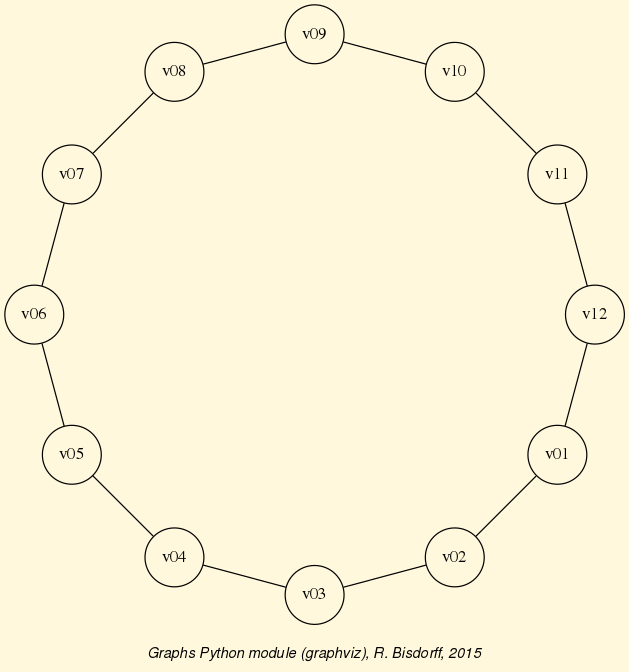
\includegraphics[width=6cm]{Figures/cg12.png}
\caption{The 12-cycle graph} 
\label{fig:24.1}       % Give a unique label
\end{figure}

\section{Computing maximal independent sets (MISs)}
\label{sec:24.1}
---------------------------------------------

A non isomorphic MIS corresponds in fact to a set of isomorphic MISs, i.e. an orbit of MISs under the automorphism group of the 12-cycle graph. We are now first computing all maximal independent sets that are detectable in the 12-cycle digraph with the \texttt{showMIS()} method.
\begin{lstlisting}
>>> c12.showMIS(withListing=False)
  *---  Maximal independent choices ---*
   number of solutions:  29
   cardinality distribution
   card.:  [0, 1, 2, 3, 4,  5,  6, 7, 8, 9, 10, 11, 12]
   freq.:  [0, 0, 0, 0, 3, 24,  2, 0, 0, 0,  0,  0,  0]
   Results in c12.misset
\end{lstlisting}
In the 12-cycle graph, we observe 29 labelled MISs: 3 of cardinality 4, 24 of cardinality 5, and 2  of cardinality 6. In case of n-cycle graphs with $n$ > 20, as the cardinality of the MISs becomes big, it is preferable to use the shell \texttt{perrinMIS} command compiled from C and installed  along with all the \Digraph python modules for computing the set of MISs observed in the graph\footnote{The \texttt{perrinMIS} shell command may be installed system wide with the command texttt{make installPerrin} from the main \Digraph directory. It is stored by default into \texttt{/usr/local/bin/}. This may be changed with the \texttt{INSTALLDIR} flag. The command \texttt{make installPerrinUser} installs it instead without sudo into the user's private \texttt{.bin} directory.}.
\begin{lstlisting}
...$ echo 12 | /usr/local/bin/perrinMIS
  # $------------------------------------- #
  # Generating MIS set of Cn with the      #
  # Perrin sequence algorithm.             #
  # Temporary files used.                  #
  # even versus odd order optimised.       #
  # RB December 2006                       #
  # Current revision Dec 2018              #
  # -------------------------------------- #
  Input cycle order ? <-- 12
   mis 1 : 100100100100
   mis 2 : 010010010010
   mis 3 : 001001001001
    ...
    ...
    ...
   mis 27 : 001001010101
   mis 28 : 101010101010
   mis 29 : 010101010101
   Cardinalities:
   0 : 0
   1 : 0
   2 : 0
   3 : 0
   4 : 3
   5 : 24
   6 : 2
   7 : 0
   8 : 0
   9 : 0
   10 : 0
   11 : 0
   12 : 0
   Total: 29
   execution time: 0 sec. and 2 millisec.
\end{lstlisting}
Reading in the result of the \texttt{perrinMIS} shell command, stored in a file called by default \texttt{curd.dat}, may be operated with the \texttt{readPerrinMisset()} method.
\begin{lstlisting}
>>> c12.readPerrinMisset(file='curd.dat')
>>> c12.misset
    {frozenset({'5', '7', '10', '1', '3'}),
     frozenset({'9', '11', '5', '2', '7'}),
     frozenset({'7', '2', '4', '10', '12'}),
     ...
     ...
     ...
     frozenset({'8', '4', '10', '1', '6'}),
     frozenset({'11', '4', '1', '9', '6'}),
     frozenset({'8', '2', '4', '10', '12', '6'})
    }
\end{lstlisting}

\section{Computing the automorphism group}
\label{sec:24.2}

For computing the corresponding non isomorphic MISs, we actually need the automorphism group of the c12-cycle graph. The \texttt{Digraph} class therefore provides the \texttt{automorphismGenerators()} method which adds automorphism group generators to a \texttt{Digraph} class instance with the help of the external shell \texttt{dreadnaut} command from the \emph{nauty} software package \footnote{The \texttt{automorphismGenerators} method uses the \texttt{dreadnaut} shell command from the \emph{nauty} software package. See https://www3.cs.stonybrook.edu/~algorith/implement/nauty/implement.shtml . On Mac OS there exist dmg installers and on Ubuntu Linux or Debian, one may easily install it with \texttt{...\$ sudo apt-get install nauty}.}.
\begin{lstlisting}
>>> c12.automorphismGenerators()
      ...
    Permutations
    {'1':'1', '2':'12', '3':'11', '4':'10',
     '5':'9', '6':'8', '7':'7', '8':'6', '9':'5',
     '10':'4', '11':'3', '12':'2'}
    {'1':'2', '2':'1', '3':'12', '4':'11', '5':'10', 
     '6':'9', '7':'8', '8':'7', '9':'6', '10':'5', 
     '11':'4', '12':'3'}
>>> print('grpsize = ', c12.automorphismGroupSize)
   grpsize = 24
\end{lstlisting}
The 12-cycle graph automorphism group is generated with both the permutations above and has group size 24.

\section{Computing the isomorphic MISs}
\label{sec:24.3}

The \texttt{showOrbits()} method renders now the labelled representatives of each of the four orbits of isomorphic MISs observed in the 12-cycle graph (see Lines 7-10 below).
\begin{lstlisting}
>>> c12.showOrbits(c12.misset,withListing=False)
    ...
  *---- Global result ----
   Number of MIS:  29
   Number of orbits :  4
   Labelled representatives and cardinality:
   1: ['2','4','6','8','10','12'], 2
   2: ['2','5','8','11'], 3
   3: ['2','4','6','9','11'], 12
   4: ['1','4','7','9','11'], 12
   Symmetry vector
   stabilizer size: [1, 2, 3, ..., 8, 9, ..., 12, 13, ...]
   frequency      : [0, 2, 0, ..., 1, 0, ...,  1,  0, ...]
\end{lstlisting}
The corresponding group stabilizers' sizes and frequencies: orbit 1 with 6 symmetry axes, orbit 2 with 4 symmetry axes, and orbits 3 and 4 both with one symmetry axis (see Lines 12-13 above), are illustrated in the corresponding unlabelled graphs of Fig. \ref{fig:24.1} below.
\begin{figure}[h]
\sidecaption
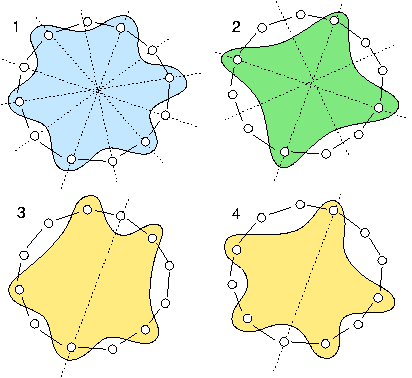
\includegraphics[width=6cm]{Figures/c12.png}
\caption{The symmetry axes of the four non isomorphic MISs of the 12-cycle graph} 
\label{fig:24.2}       % Give a unique label
\end{figure}

The non isomorphic MISs in the 12-cycle graph represent in fact all the ways one may write the number 12 as the circular sum of '2's and '3's without distinguishing opposite directions of writing. The first orbit corresponds to writing six times a '2'; the second orbit corresponds to writing four times a '3'. The third and fourth orbit correspond to writing two times a '3' and three times a '2'. There are two non isomorphic ways to do this latter circular sum. Either separating the '3's by one and two '2's, or by zero and three '2's (see Bisdorff \& Marichal [ISOMIS-08]).
 
